\documentclass[8pt,a4paper,landscape]{extarticle}
% -- Layout ----
\usepackage[top=0.6cm, bottom=0.6cm, left=0.5cm, right=0.5cm, landscape]{geometry}

% -- Titles ----
\usepackage[
  tiny,                     % text size title
  compact                   % reduce vertical space before/after title
]{titlesec}
% \titlespacing*
\titleformat{\section}{\normalfont\small\bfseries}{\thesection}{0em}{} % Remove space before and after section titles
\titleformat{\subsection}{\normalfont\small\bfseries}{\thesubsection}{0em}{} % Remove space before and after subsection titles
\titlespacing*{\section}{0pt}{0pt}{0pt} % Remove space before/after section titles
\titlespacing*{\subsection}{0pt}{0pt}{0pt} % Remove space before/after subsec titles

% -- Colors ----
\usepackage[dvipsnames]{xcolor}
\definecolor{dmm}{RGB}{192,192,192} % Define a custom dimmed text color
\definecolor{cmt}{RGB}{61,123,123}

% -- Math ------
\usepackage{mathtools}
\usepackage{amssymb}
\usepackage{turnstile}%better vdash

% -- Lists -----
\usepackage[inline]{enumitem}
\setlist{noitemsep}% Remove vspace between items
% Set vspace before and after  list environments as well as the left margin
\setlist[itemize,1]{leftmargin=.6em,labelindent=0pt,labelsep=2pt,
  topsep=1pt,partopsep=1pt}
\setlist[enumerate,1]{leftmargin=1em,labelindent=0pt,labelsep=2pt,
  topsep=1pt,partopsep=1pt}
\setlist[itemize,2]{leftmargin=.3em,labelindent=1pt,topsep=1pt,partopsep=1pt}
\setlist[enumerate,2]{leftmargin=0.2em,labelindent=1pt,topsep=1pt,partopsep=1pt}
\setlist[description]{labelwidth=\linewidth,font=\small\bfseries,leftmargin=1em,topsep=1pt,partopsep=1pt}
% -- Code listing ---
\usepackage{listings}
\lstset{
  aboveskip=3pt,
  belowskip=3pt,
  basicstyle=\small\ttfamily,
  breaklines=true,
  % commentstyle=\upshape\ttfamily,
  captionpos=b,
  commentstyle=\color{cmt},
  columns=flexible,
  frame=single,
  keepspaces=false,
  keywordstyle=\bfseries,
  showspaces=false,
  showstringspaces=false,
  showtabs=false,
  tabsize=2,
}

% Parse Trees
\usepackage{tikz}
\usetikzlibrary{ arrows, automata, bbox, calc, positioning, tikzmark, decorations.pathmorphing, decorations.pathreplacing, decorations.shapes, }
\tikzset{
  >=stealth',
  node distance=1cm,
  recstate/.style={
    circle,draw=blue!50,fill=blue!20,thick,font=\small\sffamily,rounded corners=3pt,
    minimum size=1cm,inner sep=1pt
  },
  ivp/.style={draw,->,auto,font=\small\sffamily,bend angle=60},
  msi/.style={draw=Brown,->,auto,font=\small\sffamily,bend angle=80},
  msibs/.style={draw=RoyalBlue,->,auto,font=\small\sffamily,bend angle=80},
  msinl/.style={font=\footnotesize\sffamily}, %msi node label
  every edge/.style={draw,auto,font=\small\sffamily},
  every loop/.style={looseness=4},
  initial text=start,initial where=right
}

% Place a figure env right here via [H] option
\usepackage{float}

% Side by side figure
\usepackage{subcaption}
% \usepackage{caption}
% \captionsetup{belowskip=0pt, aboveskip=0pt}
\usepackage{pifont}

% -- Multi-Col layout --
\usepackage{multicol}

% No indentation
\setlength\parindent{0pt}
\setlength\abovedisplayskip{-5pt}
\setlength\belowdisplayskip{-5pt}
\setlength\abovedisplayshortskip{-4pt}
\setlength\belowdisplayshortskip{-4pt}
\setlength\tabcolsep{5pt}
\newcommand{\gor}{\;|\;}
\newcommand{\num}{\texttt{\#}~}
\newcommand{\pro}[1]{\textcolor{Brown}{#1}}
\newcommand{\bus}[1]{\textcolor{RoyalBlue}{#1}}
\renewcommand{\arraystretch}{1.2}


\begin{document}
% Suppress page number for all pages
\pagestyle{empty}

% Notes begin
\begin{multicols*}{3}
\section*{Jargon}
\begin{itemize}
\item \textbf{synchronous iteration}: several processes start together at the beginning of each iteration and the next iteration must wait for all processors to finish current iteration, \textbf{L2P2}
\item \textbf{SPMD}: all UEs execute the same program (Single Program, SP) in parallel, but each has its own set of data (Multiple Data). In src code, usually a proc ID is used to uniquely label a UE
\item \textbf{Motivation} for parallelism (\textbf{L1P10}-\textbf{P11}):
  \begin{enumerate}
  \item speed/performance (1h vs 1w)
  \item tackle larger-scale problems
  \item keep power consumption and heat dissipation under control
  \item more $\cdots$ (see L1P11)
  \end{enumerate}
\item \textbf{Scales} of parallelism (\textbf{L1P12})
\item \textbf{peak flops/sec}$ = \# \text{cores} \times [\# \text{sockets}] \times \# \text{flops} \times \text{freq}$ (\textbf{L2-3P3})
\item ideal \textbf{speedup} is hard due to overheads (\textbf{L1P30})
  \begin{enumerate}
  \item idling (unbalanced load, sync, serial parts, etc)
  \item splitting computation into tasks
  \item communications among processes
  \end{enumerate}
\item \textbf{speedup}: $S_p = \frac{T_{seq}}{T_{par}} (\geq 1)$ (fixed problem size \textbf{L5P2})
\item \textbf{efficiency}: $E_p = \frac{S_{p}}{p} (0 < E_p \leq 1)$ (\textbf{L5P2})
\item \textbf{embarrassingly parallel}: problem solved without communication (\textbf{L5P3, L6P2})
\item \textbf{strong scalability}: fixed problem size + increasing $\# p \rightarrow$ perf. $\downarrow$
\item \textbf{weak scalability}: increasing $\# p$ and problem size $\rightarrow$ perf. $\downarrow$
\item \textbf{communication latency} time taken to communicate a message between 2 processors in a network
\item \textbf{minimal routing} takes 1 of shortest paths (XY-routing; E-cube)
\item \textbf{non-minimal} routing route the message along a longer path to avoid network congestion
\item \textbf{deterministic} routing determines a unique path \emph{solely} based on src and dest nodes
\item \textbf{adaptive} routing uses info on network state to determine message path (\textbf{L7P3})
\end{itemize}

\section*{Amdahl's law (strong scaling law, \textbf{L5P5})}
\begin{equation}
  \label{eq:amdahl}
  S_p = \frac{T_{seq}}{T_{par}} = \frac{p}{pf + (1-f)} = \frac{1}{f + \frac{1-f}{p}}
\end{equation}
where $f$ is the serial portion that cannot be parallelized
\begin{tabular}{c|c}
  \hline
  \multicolumn{2}{l}{$S \rightarrow ? $ if run on 1000 CPU and 10\% ($f$) remains sequential} \\
  \hline
  $S_{ser} \quad p = 1$ & $S_{par} \quad p = 1000$  \\
  \hline
  2GFLOP/s  & $S_{ser} \times \frac{1}{0.1 + \frac{1-0.1}{1000}} \approx 9.91 \times S_{ser} = 19.82$ GFLOP/s \\
  \hline
\end{tabular}
\begin{tabular}{l|r}
  \hline
  \multicolumn{2}{l}{Calc $Ax=b$ where $A$ is $M \times N$ matrix} \\
  \multicolumn{2}{l}{$T_{ser} = 2MNT$ where $T$ is time for single float op} \\
  \multicolumn{2}{l}{$T_{sort} = 2M\log_2(M)T$ where sorting can only be sequential} \\
  \hline
  $T_{ser} \quad p = 1$ & $T_{par} \quad p = P \rightarrow \infty$ \\
  \hline
  $2MNT + 2M\log_2(M)T$ & $\frac{2MNT}{P} + 2M\log_2(M)T$ \\
  \hline
\end{tabular}
\begin{align*}
  S & = \frac{T_{ser}}{T_{par}} = \frac{2MNT + 2M\log_2(M)T}{\frac{2MNT}{P} + 2M\log_2(M)T} \\
    & = \frac{2MNT + 2M\log_2(M)T}{2M\log_2(M)T} \quad (P \rightarrow \infty \therefore \frac{2MNT}{P} \rightarrow 0) \\
    & = \frac{N}{\log_2(M)} + 1
\end{align*}
\section*{Gustafson's law (weak scaling law, \textbf{L5P7})}
\(S_p = p - f(p-1)\) where $f$ is the serial portion (independent of $p$ and problem size) and has the following assumptions:
\begin{enumerate}
\item the serial portion is kept constant when scaling problem size ($N$)
\item the perfectly parallelizable portion scales linearly with $\#p$ if $N$ scales linearly, then $T_{par}$ is kept constant.
\end{enumerate}

\section*{Moore's Law and Dennard Scaling (\textbf{L1P17})}

\begin{itemize}
  \item the two laws (\emph{underpin} exponential perf. increase of microprocessors)
  \item \textbf{Moore's} law (transistors doubles $\ne$ perf. doubles, \textbf{L1P17})
  \item \textbf{Dennard} Scaling (\textbf{L1P18-19}, examples below)
  \item[] $P = QfCV^{2}$ ($Q$: \# of transistors, $f$ frequency)
  \begin{tabular}{c|ccc}
    \hline
    \multicolumn{4}{l}{scale down feature size by  $\frac{1}{k}\approx 0.7$, then $k\approx 1.42, k^{2}\approx 2$} \\
    \hline
    & \# of trans. $Q$ & freq. $f$ & power usage $P$  \\
    \hline
    $Q_{0} = Q_{k}$ & unchanged & $f_k = k \cdot f_0$ & $P_k = (\frac{1}{k})P_0$\\
    $P_{0} = P_{k}$ & $Q_k = k^{2} \cdot Q_0$ & $f_k = k \cdot f_0$ & unchanged  \\
    \hline
    \multicolumn{4}{l}{feature size $\geq$ 100nm or $VI_{\text{leakage}}$  dominates power consumption} \\
    \hline
  \end{tabular}
\item these two also \emph{undermine} parallel computing however (\textbf{L1P21})
\item end of Dennard scaling $\rightarrow$ multicore era (\textbf{L1P23-24})
\end{itemize}

\section*{Flynn's Taxonomy (\textbf{L2-3P12-14})}
\begin{tabular}{l|p{4cm}l}
  \hline
  Type & Note & Example \\
  \hline
  SISD & 1 ix process a stream data  & von Neumann model \\
  SIMD & 1 ix stream broadcast to many & vector processor; Quardrics\\
  MISD & no such machines  & - \\
  MIMD & each proc with its own ix/data & Gadi; most of top 500 \\
  \hline
\end{tabular}

\section*{Store-and-Forward (SF) routing (\textbf{L7P5})}
\begin{equation*}
  t_{\text{comm}} = t_{s} + l(t_h + mt_w) \quad m \text{ is message size}; l \text{ is link num}
\end{equation*}
\begin{equation*}
  t_{\text{comm}} \approx t_{s} + lmt_w (\because t_h \ll mt_w \text{even for small} m)
\end{equation*}
\section*{Cut-Through (CT) routing (\textbf{L7P6})}
\begin{equation*}
  t_{\text{comm}} = t_{s} + lt_h + mt_w
\end{equation*}
If the communication is between nearest neighbors (that is, $l = 1$), or if the message size is small, then $T_{\text{comm}}$ is similar for store-and-forward and cut-through routing
\section*{One-to-all SF on different networks (\textbf{L7P9-10})}
\begin{tabular}{c|lc}
  \hline
  Network & Communication Cost & Source \\
  \hline
  Ring & $T_{\text{one-all}} = (t_s + t_{w}m) \frac{p}{2}$  & \textbf{L7P9} \\
  2D Mesh & $T_{\text{one-all}} = 2(t_s + t_{w}m) \frac{\sqrt{p}}{2}$ & \\
  3D Mesh & $T_{\text{one-all}} = 3(t_s + t_{w}m) \frac{\sqrt[3]{p}}{2}$ &  \\
  Hypercude & $T_{\text{one-all}} = (t_s + t_{w}m) \log_2 p$ & \textbf{L7P10} \\
  \hline
  \multicolumn{3}{l}{one-to-all broadcast with SF routing is \textbf{fastest} on hypercube}\\
  \hline
\end{tabular}
\section*{One-to-all CT on different networks (\textbf{L7P11-13})}
\begin{tabular}{c|l|c}
  \hline
  Network & Communication Cost & Source \\
  \hline
  Ring & $T_{\text{one-all}} = \log_2 p(t_s + mt_{w}) + t_h(p-1)$ & \textbf{L7P11} \\
  2D Mesh & $T_{\text{one-all}} = 2\log_2 (\sqrt{p})(t_s + mt_{w}) + 2t_h(\sqrt{p}-1) $ & \textbf{L7P12}\\
  Binary Tree & $T_{\text{one-all}} = \log_2(p)(t_s + mt_{w})+(\sum^{\log_2(p)}_{i=1}2i)t_h$ & \textbf{L7P13} \\
  \hline
  \multicolumn{3}{l}{one-to-all broadcast with CF does \emph{not} improve (not faster than SF)}\\
  \multicolumn{3}{l}{because of exclusively nearest-neighbor communication}\\
  \hline
\end{tabular}

\section*{All-to-All Store-and-Forward (SF) Routing (\textbf{L7P14-16})}
\begin{tabular}{c|l|c}
  \hline
  Network & Communication Cost & Source \\
  \hline
  Ring & $T_{\text{all-all}} = (p-1)(t_s + t_h mt_{w})$ & \textbf{L7P14} \\
  2D Torus & $T_{\text{all-all}} = 2(t_s + t_h)(\sqrt{p} - 1)+mt_{w}(p-1)$ & \textbf{L7P15}\\
  Hypercube & $T_{\text{all-all}} = 2\log_2(p)(t_s + t_h)+2(p-1)mt_w$ & \textbf{L7P16} \\
  \hline
\end{tabular}

\section*{Methods for containing interaction overheads}
\begin{enumerate}
\item Maximizing Data Locality
  \begin{itemize}
  \item Minimize Volume of Data-Exchange (minimize the overall volume of shared data, akin to maximizing the temporal data locality)
  \item Minimize Frequency of Interaction (there is a relatively high startup cost associated with each interaction on many architectures)
  \end{itemize}
\item Minimizing Contention and Hot Spots
\item Overlapping Computations with Interactions (init interaction early enough so that it's completed before it's needed for computation)
\item Replicating Data or Computations
\item Using Optimized Collective Interaction Operations
\item Overlapping Interactions with Other Interactions
\end{enumerate}
\section*{Parallel Algorithm Models}
\begin{itemize}
\item Data-Parallel (data parallelism, GPU) tasks are statically or semi-statically mapped onto processes and each task performs similar operations on different data
\item Task Graph: interrelationships among the tasks are utilized to promote locality or to reduce interaction costs; typically employed to solve problems in which the amount of data associated with the tasks is large relative to the amount of computation associated with them.
\item Work Pool: a dynamic mapping of tasks onto processes for load balancing in which any task may potentially be performed by any process; no desired premapping of tasks onto processes
\item Master-Slave (manager-worker): one or more master processes generate work and allocate it to worker processes
\item Pipeline or Producer-Consumer: a stream of data is passed on through a succession of processes, each of which perform some task on it
\end{itemize}


% \section*{Matrices Multiplication (Square n $\times$ n)}
\begin{equation*}
  A_{n,n} \times B_{n,n} =
 \begin{bmatrix}
  a_{11} & a_{12} & \cdots & a_{1n} \\
  a_{21} & a_{22} & \cdots & a_{2n} \\
  \vdots  & \vdots  & \ddots & \vdots  \\
  a_{n1} & a_{n2} & \cdots & a_{nn}
 \end{bmatrix}
  \begin{bmatrix}
  b_{11} & b_{12} & \cdots & b_{1n} \\
  b_{21} & b_{22} & \cdots & b_{2n} \\
  \vdots  & \vdots  & \ddots & \vdots  \\
  b_{n1} & b_{n2} & \cdots & b_{nn}
 \end{bmatrix}
\end{equation*}
\begin{align*}
  \label{eq:mmitem}
  C_{ij} & =  \begin{bmatrix}
                a_{i1} \\
                a_{i2} \\
                \vdots \\
                a_{in}
              \end{bmatrix}
              \begin{bmatrix}
                b_{1j} & b_{2j} & \cdots & b_{nj}
              \end{bmatrix} =
           \begin{bmatrix}
                a_{i1} \\
                a_{i2} \\
                \vdots \\
                a_{in}
           \end{bmatrix}
           \cdot
           \begin{bmatrix}
                b_{1j} \\
                b_{2j} \\
                \vdots \\
                b_{nj}
           \end{bmatrix} \\
         & = a_{i1}\cdot b_{1j}+a_{i2}\cdot b_{2j}+\cdots+a_{in}\cdot b_{nj} \\
         & = \sum_{i,j=1}^{n}a_{ij}\cdot b_{ji}
\end{align*}

\lstinputlisting[language=C,linerange={4-17}]{sec/matrixmul1.c}

\section*{Mapping 2D array to 1D array in \texttt{C}}
\begin{itemize}
\item given a grid of size $M$ by $N$ where $M$ is row $\#$ and $N$ is column $\#$
\item halo layer around only 4 edges: top, bottom, left, right
\item corner elements of halo: (0,0), (0,$N+1$), ($M+1$,$N+1$), ($M+1$,0)
\item corner elements of interior field: (1,1), (1,$N$), ($M,N$), ($M$,1)
\item using 1D array \texttt{u[]} to store all points, thus \texttt{u} size $(M+2)\times(N+2)$
\item parallel algorithm implementation on $P$ by $Q$ process grid
\item use a 2-stage halo exchange: top-bottom then left-right
\end{itemize}
% M by N matrix
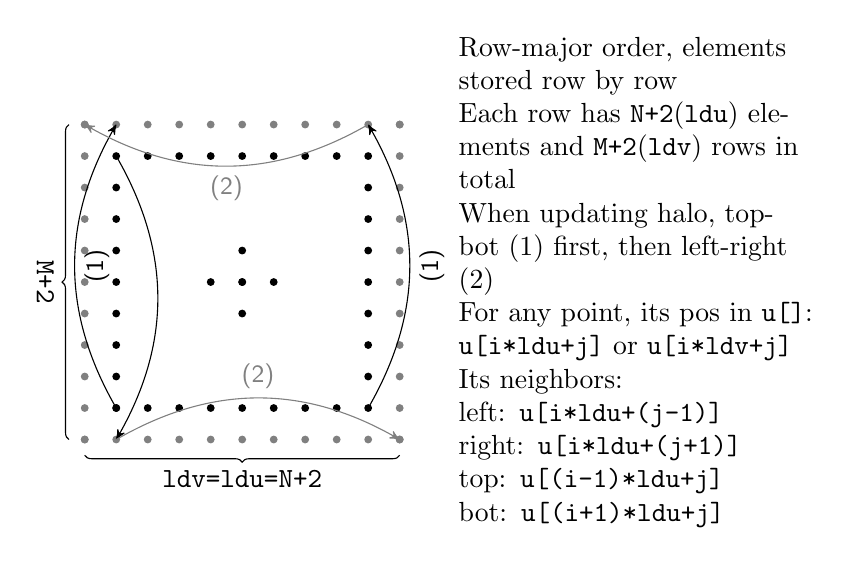
\begin{tikzpicture}
  [halo/.style={circle,fill,gray,inner sep=1pt},
  innr/.style={circle,fill,inner sep=1pt},
  info/.style={inner sep=1ex,font=\small}]

  % halo
  \foreach \i in {0,0.4,...,4} {
    \node at (\i,0)[halo]{}; %halo top
    \node at (\i,4)[halo]{}; %halo bot
    \node at (0,\i)[halo]{}; %halo left
    \node at (4,\i)[halo]{}; %halo right
  }

  % halo
  \foreach \j in {0.4,0.8,...,3.6} {
    \node at (\j,3.6)[innr]{}; %inner top
    \node at (\j,0.4)[innr]{}; %inner bot
    \node at (0.4,\j)[innr]{}; %inner left
    \node at (3.6,\j)[innr]{}; %inner right
  }
  \node at (3.6,3.6)[innr]{};

  \foreach \m in {1.6,2.0,2.4} {
    \node at (\m, 2.0)[innr]{};
    \node at (2.0, \m)[innr]{};
  }

  % neighbors

  \draw[decorate,decoration={brace,mirror}] (-.2,4.0) -- (-.2,0); %left
  \draw[decorate,decoration={brace,mirror}] (0,-.2) -- (4.0,-.2); %bot
  \node at (-.5,2)[rotate=-90]{\texttt{M+2}};
  \node at (2,-.5)[](ldu){\texttt{ldv=ldu=N+2}};

  % halo src to dest
  \path[->] (0.4,0.4) edge[bend left] node[below,sloped]{(1)} (0.4,4); %top halo left
  \path[->] (3.6,0.4) edge[bend right] node[below,sloped]{(1)} (3.6,4);%top halo right
  \path[->] (0.4,3.6) edge[bend left] (0.4,0);

  \path[->] (3.6,4) edge[bend left,gray] node[below,sloped]{(2)} (0,4);
  \path[->] (0.4,0) edge[bend left,gray] node[above,sloped]{(2)} (4,0);

  % txt
  \node[xshift=7cm,yshift=2cm,text width=4.5cm]
  {
    Row-major order, elements stored row by row\\
    Each row has \texttt{N+2}(\texttt{ldu}) elements and \texttt{M+2}(\texttt{ldv}) rows in total\\
    When updating halo, top-bot (1) first, then left-right (2) \\
    For any point, its pos in \texttt{u[]}:
    \texttt{u[i*ldu+j]} or \texttt{u[i*ldv+j]}\\
    Its neighbors:\\
    left:  \texttt{u[i*ldu+(j-1)]} \\
    right: \texttt{u[i*ldu+(j+1)]}\\
    top:   \texttt{u[(i-1)*ldu+j]}\\
    bot:   \texttt{u[(i+1)*ldu+j]}
  };
\end{tikzpicture}
      % top left halo, \texttt{u[1] = u[(M+1)*ldu+1]}\\
      % top right halo, \texttt{u[1] = u[(M+1)*ldu+1]}\\
      % bot left halo, \texttt{u[1] = u[(M+1)*ldu+1]}\\
      % bot right halo, \texttt{u[1] = u[(M+1)*ldu+1]}\\
      % left halo, \texttt{u[1] = u[(M+1)*ldu+1]}\\
      % right halo, \texttt{u[1] = u[(M+1)*ldu+1]}\\

\section*{Overhead and resolution of timer}
\begin{itemize}
\item Overhead = $\text{Avg}(\text{overhead}_1,\text{overhead}_2,\cdots,\text{overhead}_n)$
\item Resolution = Smallest diff between any 2 watched times
\end{itemize}
\end{multicols*}
\end{document}
